% questions.tex —— 2011 年·陕西卷·理科 · 题目内容片段（无答案）
% 由 tools/generate_projects.py 依来源总账自 2011/2011_数学真题_陕西理_试题.md 生成，勿手改（改源 MD 后重跑）

\gkpart{一、选择题}

\begin{question}
\gkti{1}设 $\boldsymbol a$，$\boldsymbol b$ 是向量，命题“若 $\boldsymbol a=-\boldsymbol b$，则 $|\boldsymbol a|=|\boldsymbol b|$”的逆命题是\mbox{（　　）}

（A）若 $\boldsymbol a\ne-\boldsymbol b$，则 $|\boldsymbol a|\ne|\boldsymbol b|$

（B）若 $\boldsymbol a=-\boldsymbol b$，则 $|\boldsymbol a|\ne|\boldsymbol b|$

（C）若 $|\boldsymbol a|\ne|\boldsymbol b|$，则 $\boldsymbol a\ne-\boldsymbol b$

（D）若 $|\boldsymbol a|=|\boldsymbol b|$，则 $\boldsymbol a=-\boldsymbol b$

\end{question}
\begin{question}
\gkti{2}设抛物线的顶点在原点，准线方程为 $x=-2$，则抛物线的方程是\mbox{（　　）}

（A）$y^2=-8x$

（B）$y^2=-4x$

（C）$y^2=8x$

（D）$y^2=4x$

\Needspace{0.4\textheight}
\end{question}
\begin{question}
\gkti{3}设函数 $f(x)$（$x\in\mathbf R$）满足 $f(-x)=f(x)$，$f(x+2)=f(x)$，则 $y=f(x)$ 的图象可能是\mbox{（　　）}
\nopagebreak[4]
\begin{center}% 2011 年陕西卷理科第 3 题：四个函数图象（A 奇函数；B 偶函数且周期 2；C 奇函数；D 偶函数但周期 4）。
% 来源 PDF：普通高考/2011/2011陕西理.pdf，SHA-256 04dab6de0e3ee6223a1cbc126f7f83ae354d2b31201a14db1f31c8477d8a3bed。
% 原页：第 1 页第 1 栏中部，书页码 693。
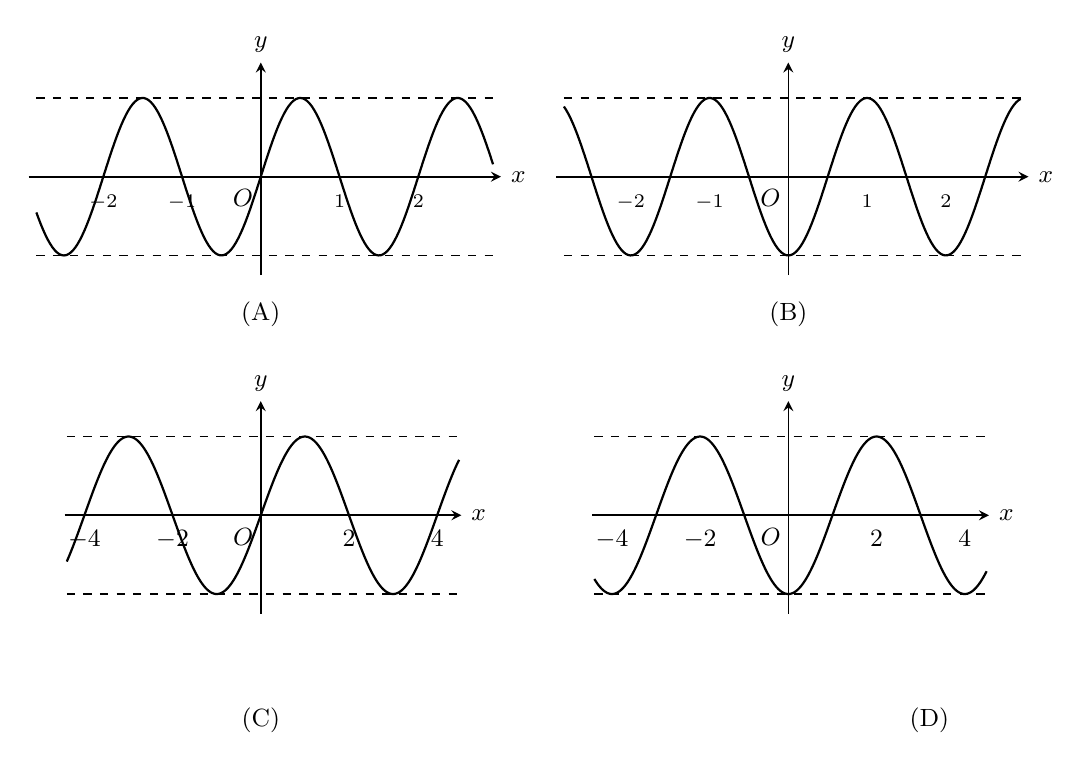
\begin{tikzpicture}[>=stealth, semithick, font=\small]
  % (A) y=sin(pi x)：过原点，奇函数
  \begin{scope}
    \draw[->] (-2.95,0)--(3.05,0) node[right] {$x$};
    \draw[->] (0,-1.25)--(0,1.45) node[above] {$y$};
    \draw[dashed] (-2.85,1)--(2.95,1) (-2.85,-1)--(2.95,-1);
    \draw[thick, domain=-2.85:2.95, samples=200] plot (\x,{sin(180*\x)});
    \foreach \t in {-2,-1,1,2} {\node[below,font=\scriptsize] at (\t,-0.10) {$\t$};}
    \node[below left] at (0.03,-0.04) {$O$};
    \node at (0,-1.75) {(A)};
  \end{scope}
  % (B) y=-cos(pi x)：偶函数，周期 2
  \begin{scope}[xshift=6.7cm]
    \draw[->] (-2.95,0)--(3.05,0) node[right] {$x$};
    \draw[->] (0,-1.25)--(0,1.45) node[above] {$y$};
    \draw[dashed] (-2.85,1)--(2.95,1) (-2.85,-1)--(2.95,-1);
    \draw[thick, domain=-2.85:2.95, samples=200] plot (\x,{-cos(180*\x)});
    \foreach \t in {-2,-1,1,2} {\node[below,font=\scriptsize] at (\t,-0.10) {$\t$};}
    \node[below left] at (0.03,-0.04) {$O$};
    \node at (0,-1.75) {(B)};
  \end{scope}
  % (C) y=sin(pi x/2)：过原点，奇函数
  \begin{scope}[yshift=-4.3cm, xscale=0.56]
    \draw[->] (-4.45,0)--(4.55,0) node[right] {$x$};
    \draw[->] (0,-1.25)--(0,1.45) node[above] {$y$};
    \draw[dashed] (-4.4,1)--(4.5,1) (-4.4,-1)--(4.5,-1);
    \draw[thick, domain=-4.4:4.5, samples=300] plot (\x,{sin(90*\x)});
    \foreach \t in {-4,-2,2,4} {\node[below] at (\t,-0.06) {$\t$};}
    \node[below left] at (0.06,-0.04) {$O$};
    \node at (0,-2.6) {(C)};
  \end{scope}
  % (D) y=-cos(pi x/2)：偶函数，周期 4
  \begin{scope}[yshift=-4.3cm, xshift=6.7cm, xscale=0.56]
    \draw[->] (-4.45,0)--(4.55,0) node[right] {$x$};
    \draw[->] (0,-1.25)--(0,1.45) node[above] {$y$};
    \draw[dashed] (-4.4,1)--(4.5,1) (-4.4,-1)--(4.5,-1);
    \draw[thick, domain=-4.4:4.5, samples=300] plot (\x,{-cos(90*\x)});
    \foreach \t in {-4,-2,2,4} {\node[below] at (\t,-0.06) {$\t$};}
    \node[below left] at (0.06,-0.04) {$O$};
    \node at (3.2,-2.6) {(D)};
  \end{scope}
\end{tikzpicture}
\end{center}
\nopagebreak[4]
\end{question}
\begin{question}
\gkti{4}$(4^x-2^{-x})^6$（$x\in\mathbf R$）展开式中的常数项是\mbox{（　　）}

（A）$-20$

（B）$-15$

（C）$15$

（D）$20$

\Needspace{0.4\textheight}
\end{question}
\begin{question}
\gkti{5}某几何体的三视图如图所示，则它的体积是\mbox{（　　）}

（A）$8-\frac{2\pi}3$

（B）$8-\frac{\pi}3$

（C）$8-2\pi$

（D）$\frac{2\pi}3$
\nopagebreak[4]
\begin{center}% 2011 年陕西卷理科第 5 题：正方体挖去圆锥的三视图。
% 来源 PDF：普通高考/2011/2011陕西理.pdf，SHA-256 04dab6de0e3ee6223a1cbc126f7f83ae354d2b31201a14db1f31c8477d8a3bed。
% 原页：第 1 页第 1 栏下部，书页码 693。外形 2×2×2，俯视图内切圆半径 1。
\begin{tikzpicture}[semithick, font=\small, scale=0.85]
  % 主视图
  \draw[thick] (0,0) rectangle (2,2);
  \draw[dashed] (0,2)--(1,0.35)--(2,2);
  \node at (1,-0.42) {主视图};
  \draw[<->] (0,2.42)--(2,2.42) node[midway, above] {$2$};
  % 主视图宽度标注
  % 左视图
  \begin{scope}[xshift=3.6cm]
    \draw[thick] (0,0) rectangle (2,2);
    \draw[dashed] (0,2)--(1,0.35)--(2,2);
    \node at (1,-0.42) {左视图};
    \draw[<->] (2.4,0)--(2.4,2) node[midway, right] {$2$};
  \end{scope}
  % 俯视图
  \begin{scope}[yshift=-3.6cm]
    \draw[thick] (0,0) rectangle (2,2);
    \draw[thick] (1,1) circle (1);
    \node at (1,-0.42) {俯视图};
  \end{scope}
\end{tikzpicture}
\end{center}
\nopagebreak[4]
\end{question}
\begin{question}
\gkti{6}函数 $f(x)=\sqrt x-\cos x$ 在 $[0,+\infty)$ 内\mbox{（　　）}

（A）没有零点

（B）有且仅有一个零点

（C）有且仅有两个零点

（D）有无穷多个零点

\end{question}
\begin{question}
\gkti{7}设集合 $M=\left\{y\mid y=|\cos^2x-\sin^2x|,\ x\in\mathbf R\right\}$，$N=\left\{x\mid\left|x-\dfrac1{\mathrm i}\right|<\sqrt2,\ x\in\mathbf R\right\}$（$\mathrm i$ 为虚数单位），则 $M\cap N$ 为\mbox{（　　）}

（A）$(0,1)$

（B）$(0,1]$

（C）$[0,1)$

（D）$[0,1]$

\Needspace{0.4\textheight}
\end{question}
\begin{question}
\gkti{8}如图，$x_1$，$x_2$，$x_3$ 为某次考试三个评阅人对同一道题的独立评分，$p$ 为该题的最终得分，当 $x_1=6$，$x_2=9$，$p=8.5$ 时，$x_3$ 等于\mbox{（　　）}

（A）$11$

（B）$10$

（C）$8$

（D）$7$
\nopagebreak[4]
\begin{center}% 2011 年陕西卷理科第 8 题：评分程序框图。
% 来源 PDF：普通高考/2011/2011陕西理.pdf，SHA-256 04dab6de0e3ee6223a1cbc126f7f83ae354d2b31201a14db1f31c8477d8a3bed。
% 原页：第 1 页第 2 栏上部，书页码 693。
\begin{tikzpicture}[>=stealth, semithick, font=\small, node distance=5mm]
  \node[draw, rounded corners=0.1cm, minimum width=1.3cm, minimum height=0.45cm] (start) {开始};
  \node[draw, trapezium, trapezium left angle=72, trapezium right angle=108,
        minimum width=2.4cm, minimum height=0.5cm, below=of start] (in12) {输入 $x_1$，$x_2$};
  \node[draw, diamond, aspect=2.6, minimum width=2.6cm, minimum height=0.9cm, below=of in12] (d1) {$|x_1-x_2|\leqslant2$};
  \node[draw, trapezium, trapezium left angle=72, trapezium right angle=108,
        minimum width=2.0cm, minimum height=0.5cm, below=of d1] (in3) {输入 $x_3$};
  \node[draw, diamond, aspect=3.0, minimum width=3.4cm, minimum height=1.0cm, below=of in3] (d2) {$|x_3-x_1|<|x_3-x_2|$};
  \node[draw, minimum width=1.5cm, minimum height=0.45cm, below left=8mm and 14mm of d2] (s2) {$x_2=x_3$};
  \node[draw, minimum width=1.5cm, minimum height=0.45cm, below right=8mm and 2mm of d2] (s1) {$x_1=x_3$};
  \node[draw, minimum width=2.4cm, minimum height=0.7cm, below=26mm of d2] (p) {$p=\dfrac{x_1+x_2}2$};
  \node[draw, trapezium, trapezium left angle=72, trapezium right angle=108,
        minimum width=1.8cm, minimum height=0.5cm, below=of p] (out) {输出 $p$};
  \node[draw, rounded corners=0.1cm, minimum width=1.3cm, minimum height=0.45cm, below=of out] (stop) {结束};
  \draw[->] (start)--(in12);
  \draw[->] (in12)--(d1);
  \draw[->] (d1)--node[right=2pt] {否} (in3);
  \draw[->] (in3)--(d2);
  \draw[->] (d2.west) -| node[pos=0.25, above] {是} (s2);
  \draw[->] (d2.east) -| node[pos=0.25, above] {否} (s1);
  \draw[->] (s2.south) |- (p.west);
  \draw[->] (s1.south) |- (p.east);
  \draw[->] (p)--(out);
  \draw[->] (out)--(stop);
  \draw[->] (d1.east) -- ++(2.6,0) node[pos=0.55, above] {是} |- (p.east);
\end{tikzpicture}
\end{center}
\nopagebreak[4]
\Needspace{0.4\textheight}
\end{question}
\begin{question}
\gkti{9}设 $(x_1,y_1)$，$(x_2,y_2)$，$\cdots$，$(x_n,y_n)$ 是变量 $x$ 和 $y$ 的 $n$ 个样本点，直线 $l$ 是由这些样本点通过最小二乘法得到的线性回归直线（如图），以下结论中正确的是\mbox{（　　）}

（A）$x$ 和 $y$ 的相关系数为直线 $l$ 的斜率

（B）$x$ 和 $y$ 的相关系数在 $0$ 到 $1$ 之间

（C）当 $n$ 为偶数时，分布在 $l$ 两侧的样本点的个数一定相同

（D）直线 $l$ 过点 $(\bar x,\bar y)$
\nopagebreak[4]
\begin{center}% 2011 年陕西卷理科第 9 题：散点图与最小二乘回归直线。
% 来源 PDF：普通高考/2011/2011陕西理.pdf，SHA-256 04dab6de0e3ee6223a1cbc126f7f83ae354d2b31201a14db1f31c8477d8a3bed。
% 原页：第 1 页第 2 栏中部，书页码 693。
\begin{tikzpicture}[>=stealth, semithick, font=\small, scale=0.95]
  \draw[->] (-0.4,0)--(4.6,0) node[right] {$x$};
  \draw[->] (0,-0.4)--(0,3.6) node[above] {$y$};
  \node[below left] at (0.02,-0.02) {$O$};
  \draw[thick] (0.35,3.0)--(4.2,0.55) node[pos=0.42, above left] {$l$};
  \foreach \p in {(0.7,2.55),(1.2,2.25),(1.7,1.95),(2.1,2.3),(2.5,1.55),(3.0,1.65),(3.3,1.05),(3.7,0.95),(4.0,0.55)}
    \fill \p circle (1.2pt);
\end{tikzpicture}
\end{center}
\nopagebreak[4]
\end{question}
\begin{question}
\gkti{10}甲、乙两人一起去游“2011 西安世园会”，他们约定，各自独立地从 $1$ 到 $6$ 号景点中任选 $4$ 个进行游览，每个景点参观 $1$ 小时，则最后一小时他们在同一个景点的概率是\mbox{（　　）}

（A）$\frac1{36}$

（B）$\frac19$

（C）$\frac5{36}$

（D）$\frac16$

\end{question}
\gkpart{二、填空题}

\begin{question}
\gkti{11}设 $f(x)=\begin{cases}\lg x,&x>0,\\[2pt]x+\displaystyle\int_0^a3t^2\,\mathrm dt,&x\leqslant0.\end{cases}$ 若 $f(f(1))=1$，则 $a=\underline{\qquad}$。

\end{question}
\begin{question}
\gkti{12}设 $n\in\mathbf N_+$，一元二次方程 $x^2-4x+n=0$ 有整数根的充要条件是 $n=\underline{\qquad}$。

\end{question}
\begin{question}
\gkti{13}观察下列等式

\nopagebreak[4]
\[\begin{aligned}
1&=1\\
2+3+4&=9\\
3+4+5+6+7&=25\\
4+5+6+7+8+9+10&=49\\
&\cdots
\end{aligned}\]

照此规律，第 $n$ 个等式应为 $\underline{\qquad}$。

\end{question}
\begin{question}
\gkti{14}植树节某班 $20$ 名同学在一段直线公路一侧植树，每人植一棵，相邻两棵树相距 $10$ 米，开始时需将树苗集中放置在某一树坑旁边，使每位同学从各自树坑出发前来领取树苗往返所走的路程总和最小，这个最小值为 $\underline{\qquad}$ 米。

\Needspace{0.4\textheight}
\end{question}
\begin{question}
\gkti{15}三选一。

【A】若关于 $x$ 的不等式 $|a|\geqslant|x+1|+|x-2|$ 存在实数解，则实数 $a$ 的取值范围是 $\underline{\qquad}$。

【B】如图，$\angle B=\angle D$，$AE\perp BC$，$\angle ACD=90^\circ$，且 $AB=6$，$AC=4$，$AD=12$，则 $BE=\underline{\qquad}$。
\nopagebreak[4]
\begin{center}% 2011 年陕西卷理科第 15B 题：四边形 ABCD 与 AD、BC 的交点 E。
% 来源 PDF：普通高考/2011/2011陕西理.pdf，SHA-256 04dab6de0e3ee6223a1cbc126f7f83ae354d2b31201a14db1f31c8477d8a3bed。
% 原页：第 1 页第 3 栏中部，书页码 693。
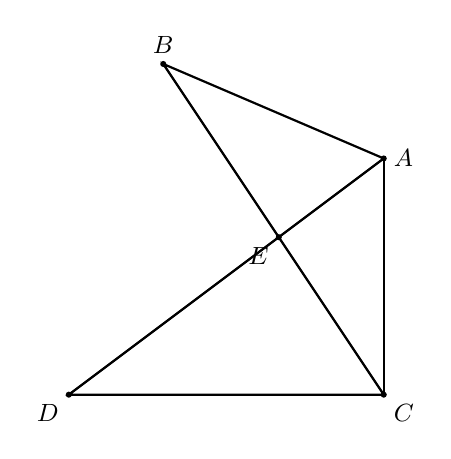
\begin{tikzpicture}[>=stealth, semithick, font=\small, scale=1.0]
  \coordinate (D) at (0,0);
  \coordinate (C) at (4,0);
  \coordinate (A) at (4,3);
  \coordinate (B) at (1.2,4.2);
  \coordinate (E) at (2.667,2.0);
  \draw[thick] (C)--(D)--(A)--(B)--(C);
  \draw[thick] (A)--(C);
  \draw (B)--(E)--(C);
  \draw (A)--(E)--(D);
  \fill (A) circle (1.1pt) node[right] {$A$};
  \fill (B) circle (1.1pt) node[above] {$B$};
  \fill (C) circle (1.1pt) node[below right] {$C$};
  \fill (D) circle (1.1pt) node[below left] {$D$};
  \fill (E) circle (1.1pt) node[below left] {$E$};
\end{tikzpicture}
\end{center}
\nopagebreak[4]
【C】直角坐标系 $xOy$ 中，以原点为极点，$x$ 轴正半轴为极轴建立极坐标系，设点 $A$，$B$ 分别在曲线 $C_1:\begin{cases}x=3+\cos\theta,\\y=4+\sin\theta,\end{cases}$（$\theta$ 为参数）和曲线 $C_2:\rho=1$ 上，则 $|AB|$ 的最小值为 $\underline{\qquad}$。

\end{question}
\gkpart{三、解答题}

\Needspace{0.4\textheight}
\begin{question}
\gkti{16}如图，在 $\triangle ABC$ 中，$\angle ABC=60^\circ$，$\angle BAC=90^\circ$，$AD$ 是 $BC$ 上的高，沿 $AD$ 把 $\triangle ABD$ 折起，使 $\angle BDC=90^\circ$。

（1） 证明：平面 $ADB\perp$ 平面 $BDC$；

（2） 设 $E$ 为 $BC$ 的中点，求 $\overrightarrow{AE}$ 与 $\overrightarrow{DB}$ 夹角的余弦值。
\nopagebreak[4]
\begin{center}% 2011 年陕西卷理科第 16 题：沿高 AD 把 △ABD 折起，使 ∠BDC=90°。左为折前，右为折后。
% 来源 PDF：普通高考/2011/2011陕西理.pdf，SHA-256 04dab6de0e3ee6223a1cbc126f7f83ae354d2b31201a14db1f31c8477d8a3bed。
% 原页：第 1 页第 3 栏下部，书页码 693。
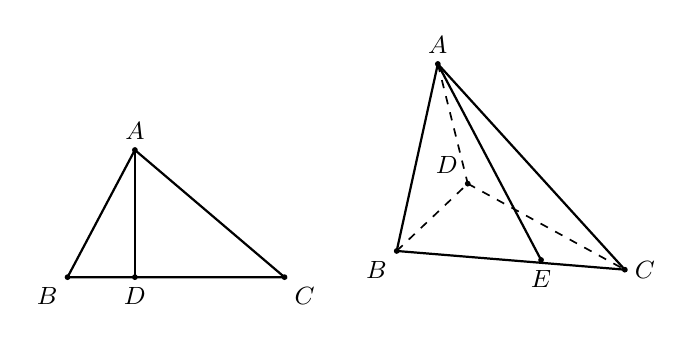
\begin{tikzpicture}[>=stealth, semithick, font=\small, scale=0.95]
  % 折前
  \coordinate (B) at (0,0);
  \coordinate (D) at (0.9,0);
  \coordinate (C) at (2.9,0);
  \coordinate (A) at (0.9,1.7);
  \draw[thick] (B)--(C)--(A)--cycle;
  \draw[thick] (A)--(D);
  \fill (A) circle (1.1pt) node[above] {$A$};
  \fill (B) circle (1.1pt) node[below left] {$B$};
  \fill (C) circle (1.1pt) node[below right] {$C$};
  \fill (D) circle (1.1pt) node[below] {$D$};
  % 折后
  \begin{scope}[xshift=4.4cm]
    \coordinate (B2) at (0,0.35);
    \coordinate (D2) at (0.95,1.25);
    \coordinate (C2) at (3.05,0.1);
    \coordinate (A2) at (0.55,2.85);
    \coordinate (E2) at (1.93,0.23);
    \draw[thick] (A2)--(B2)--(C2)--cycle;
    \draw[thick] (A2)--(E2);
    \draw[dashed] (A2)--(D2) (B2)--(D2) (D2)--(C2);
    \fill (A2) circle (1.1pt) node[above] {$A$};
    \fill (B2) circle (1.1pt) node[below left] {$B$};
    \fill (C2) circle (1.1pt) node[right] {$C$};
    \fill (D2) circle (1.1pt) node[above left] {$D$};
    \fill (E2) circle (1.1pt) node[below] {$E$};
  \end{scope}
\end{tikzpicture}
\end{center}
\nopagebreak[4]
\Needspace{0.4\textheight}
\end{question}
\begin{question}
\gkti{17}如图，设 $P$ 是圆 $x^2+y^2=25$ 上的动点，点 $D$ 是 $P$ 在 $x$ 轴上的投影，$M$ 为 $PD$ 上一点，且 $|MD|=\dfrac45|PD|$。

（1） 当 $P$ 在圆上运动时，求点 $M$ 的轨迹 $C$ 的方程；

（2） 求过点 $(3,0)$ 且斜率为 $\dfrac45$ 的直线被 $C$ 所截线段的长度。
\nopagebreak[4]
\begin{center}% 2011 年陕西卷理科第 17 题：圆 x^2+y^2=25 上的点 P，投影 D，PD 上的点 M 且 |MD|=4/5|PD|。
% 来源 PDF：普通高考/2011/2011陕西理.pdf，SHA-256 04dab6de0e3ee6223a1cbc126f7f83ae354d2b31201a14db1f31c8477d8a3bed。
% 原页：第 2 页第 1 栏上部，书页码 694。示意。
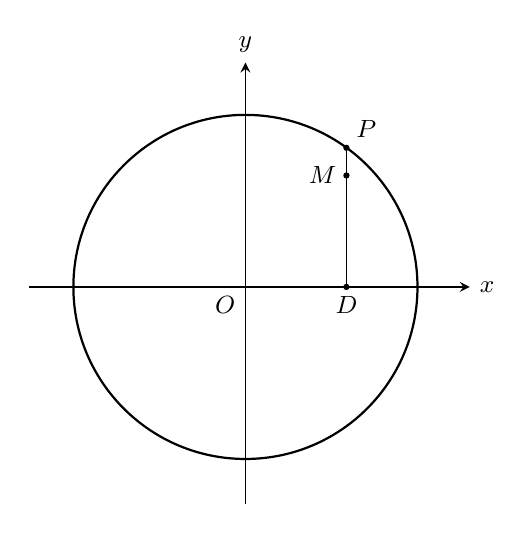
\begin{tikzpicture}[>=stealth, semithick, font=\small, scale=0.95]
  \draw[->] (-2.9,0)--(3.0,0) node[right] {$x$};
  \draw[->] (0,-2.9)--(0,3.0) node[above] {$y$};
  \draw[thick] (0,0) circle (2.3);
  \coordinate (P) at (1.35,1.86);
  \coordinate (D) at (1.35,0);
  \coordinate (M) at (1.35,1.49);
  \draw (P)--(D);
  \fill (P) circle (1.2pt) node[above right] {$P$};
  \fill (M) circle (1.2pt) node[left] {$M$};
  \fill (D) circle (1.2pt) node[below] {$D$};
  \node[below left] at (0,0) {$O$};
\end{tikzpicture}
\end{center}
\nopagebreak[4]
\end{question}
\begin{question}
\gkti{18}叙述并证明余弦定理。

\Needspace{0.4\textheight}
\end{question}
\begin{question}
\gkti{19}如图，从点 $P_1(0,0)$ 作 $x$ 轴的垂线交曲线 $y=\mathrm e^x$ 于点 $Q_1(0,1)$，曲线在 $Q_1$ 点处的切线与 $x$ 轴交于点 $P_2$，再从 $P_2$ 作 $x$ 轴的垂线交曲线于点 $Q_2$，依次重复上述过程得到一系列点：$P_1$，$Q_1$；$P_2$，$Q_2$；$\cdots$；$P_n$，$Q_n$，记 $P_k$ 点的坐标为 $(x_k,0)$（$k=1,2,\cdots,n$）。

（1） 试求 $x_k$ 与 $x_{k-1}$ 的关系（$2\leqslant k\leqslant n$）；

（2） 求 $|P_1Q_1|+|P_2Q_2|+|P_3Q_3|+\cdots+|P_nQ_n|$。
\nopagebreak[4]
\begin{center}% 2011 年陕西卷理科第 19 题：曲线 y=e^x 上点列 P_k、Q_k 与切线。
% 来源 PDF：普通高考/2011/2011陕西理.pdf，SHA-256 04dab6de0e3ee6223a1cbc126f7f83ae354d2b31201a14db1f31c8477d8a3bed。
% 原页：第 2 页第 2 栏中部，书页码 694。示意。
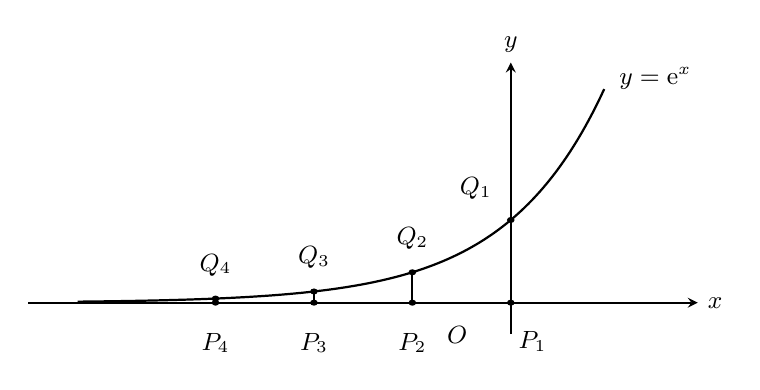
\begin{tikzpicture}[>=stealth, semithick, font=\small, xscale=1.25]
  \draw[->] (-4.9,0)--(1.9,0) node[right] {$x$};
  \draw[->] (0,-0.4)--(0,3.05) node[above] {$y$};
  \draw[thick, domain=-4.4:0.95, samples=140] plot (\x,{1.05*exp(\x)});
  \node[right] at (1.0,2.85) {$y=\mathrm e^x$};
  \foreach \k in {1,2,3,4} {
    \pgfmathsetmacro{\xk}{1-\k}
    \pgfmathsetmacro{\yk}{1.05*exp(\xk)}
    \draw[thick] (\xk,0)--(\xk,\yk);
    \fill (\xk,0) circle (1.1pt);
    \fill (\xk,\yk) circle (1.1pt);
    \ifnum\k=1\relax
      \node[below] at (0.22,-0.24) {$P_1$};
      \node[right] at (-0.62,1.45) {$Q_1$};
    \else
      \node[below] at (\xk,-0.26) {$P_{\k}$};
      \node[above] at (\xk,\yk+0.16) {$Q_{\k}$};
    \fi
  }
  \node[below left] at (-0.34,-0.18) {$O$};
\end{tikzpicture}
\end{center}
\nopagebreak[4]
\Needspace{0.4\textheight}
\end{question}
\begin{question}
\gkti{20}如图，$A$ 地到火车站共有两条路径 $L_1$ 和 $L_2$，据统计，通过两条路径所用的时间互不影响，所用时间落在各时间段内的频率如下表：

\begin{center}
\begin{tabular}{llllll}
\toprule
所用时间（分钟） & $10\sim20$ & $20\sim30$ & $30\sim40$ & $40\sim50$ & $50\sim60$ \\
\midrule
选择 $L_1$ 的人数 & $6$ & $12$ & $18$ & $12$ & $12$ \\
选择 $L_2$ 的人数 & $0$ & $4$ & $16$ & $16$ & $4$ \\
\bottomrule
\end{tabular}
\end{center}

现甲、乙两人分别有 $40$ 分钟和 $50$ 分钟时间用于赶往火车站。

（1） 为了尽最大可能在各自允许的时间内赶到火车站，甲和乙应如何选择各自的路径？

（2） 用 $X$ 表示甲、乙两人中在允许的时间内能赶到火车站的人数，针对（1）的选择方案，求 $X$ 的分布列和数学期望。
\nopagebreak[4]
\begin{center}% 2011 年陕西卷理科第 20 题：A 地到火车站的两条路径 L1、L2。
% 来源 PDF：普通高考/2011/2011陕西理.pdf，SHA-256 04dab6de0e3ee6223a1cbc126f7f83ae354d2b31201a14db1f31c8477d8a3bed。
% 原页：第 2 页第 2 栏下部，书页码 694。示意。
\begin{tikzpicture}[semithick, font=\small, scale=1.0]
  \coordinate (A) at (0,0);
  \coordinate (S) at (5.2,0);
  \draw[thick] (A) .. controls (1.7,1.15) and (3.4,0.85) .. (S);
  \draw[thick] (A) .. controls (1.7,-1.15) and (3.4,-0.85) .. (S);
  \node[below left] at (A) {$A$};
  \node[right] at (S) {火车站};
  \fill (A) circle (1.2pt);
  \fill (S) circle (1.2pt);
  \node[above] at (2.55,0.98) {$L_1$};
  \node[below] at (2.55,-0.98) {$L_2$};
\end{tikzpicture}
\end{center}
\nopagebreak[4]
\end{question}
\begin{question}
\gkti{21}设函数 $f(x)$ 定义在 $(0,+\infty)$ 上，$f(1)=0$，导函数 $f'(x)=\dfrac1x$，$g(x)=f(x)+f'(x)$。

（1） 求 $g(x)$ 的单调区间和最小值；

（2） 讨论 $g(x)$ 与 $g\left(\dfrac1x\right)$ 的大小关系；

（3） 是否存在 $x_0>0$，使得 $|g(x)-g(x_0)|<\dfrac1x$ 对任意 $x>0$ 成立？若存在，求出 $x_0$ 的取值范围；若不存在，请说明理由。

\clearpage

\end{question}